\documentclass[10pt]{beamer}

\usetheme[progressbar=frametitle]{metropolis}
\usepackage{appendixnumberbeamer}
\usepackage{multicol}
\usepackage{booktabs}
\usepackage[scale=2]{ccicons}
\usepackage[style=authoryear]{biblatex}
\bibliography{demo.bib}
\usepackage{pgfplots}


\usepgfplotslibrary{dateplot}


\usepackage{xspace}
\newcommand{\themename}{\textbf{\textsc{metropolis}}\xspace}

\title{Hospital Information Technology and Physician Response}

\subtitle{Hanna Glenn}
 \date{\today}
% \date{}
%\author{Presented by: Hanna Glenn}
% \institute{Center for modern beamer themes}
% \titlegraphic{\hfill\includegraphics[height=1.5cm]{logo.pdf}}

\begin{document}

\maketitle

\setbeamercolor{background canvas}{bg=white}

\begin{frame}{Table of Contents}
  \setbeamertemplate{section in toc}[sections numbered]
  \tableofcontents%[hideallsubsections]
\end{frame}

\section[Motivation]{Motivation}

\begin{frame}{The Beginning of HIT}
\centering
    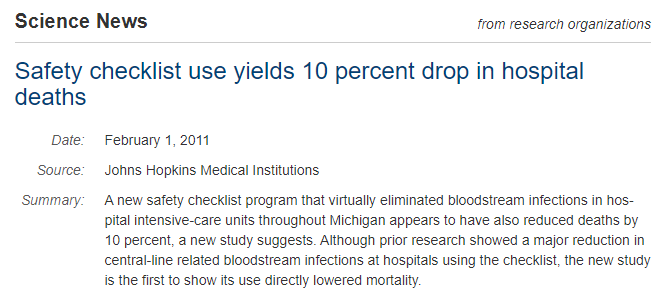
\includegraphics[scale=.6]{graphics/News Clip4.PNG}
\end{frame}

\begin{frame}[fragile]{HIT has had Great (Expected) Potential in Healthcare}
\begin{alertblock}{Cost Saving}
\begin{itemize}
    \item A 2005 estimate finds possible cost reduction of hundreds of billions of dollars (\cite{hillestad2005})
\end{itemize}
\end{alertblock}

\begin{alertblock}{Quality Improvement}
\begin{itemize}
    \item Improved efficiency, patient safety improvements, physicians have decision support that could prevent unnecessary complications, etc.
    \item Significant policy push for EHR implementation with these goal in mind: HITECH Act, 2008 provided financial incentive for hospitals to implement EHRs \nocite{hitech}
\end{itemize}
\end{alertblock}

\textcolor{blue}{The percentage of hospitals with basic EHR capability rose from 9$\%$ in 2008 to 84$\%$ in 2015.} (\cite{stats})

\end{frame}

\begin{frame}[fragile]{What does this mean for physicians?}
\begin{itemize}
    \item Day-to-day, this means physicians spend more time entering information into a computer and learning a new software
    \item Loss of autonomy as EHRs have progressed
    \item Physicians have experienced significant burn-out from EHRs
\end{itemize}

\end{frame}

\begin{frame}[noframenumbering]{Physician Burnout}
\begin{center}
    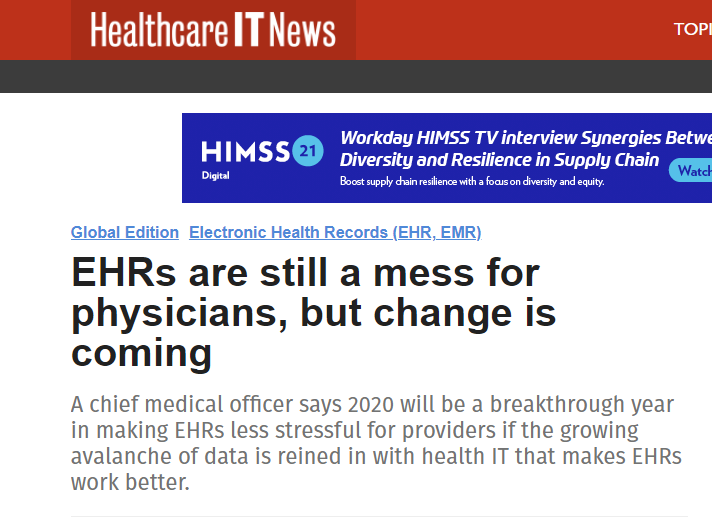
\includegraphics[scale=.4]{graphics/News Clip1.PNG}
\end{center}
\end{frame}

\begin{frame}[noframenumbering]{Physician Burnout}
\begin{center}
    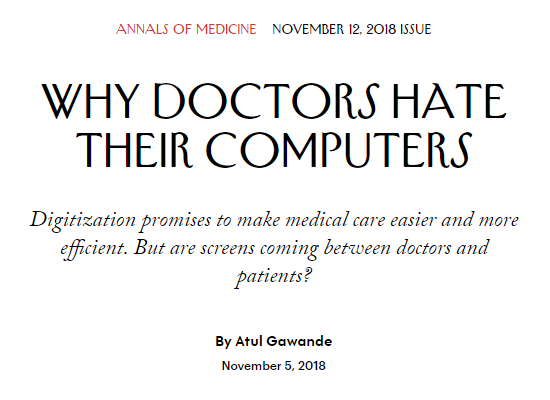
\includegraphics[scale=.5]{graphics/News Clip2.PNG}
\end{center}
\end{frame}

\begin{frame}[noframenumbering]{Physician Burnout}
\begin{center}
    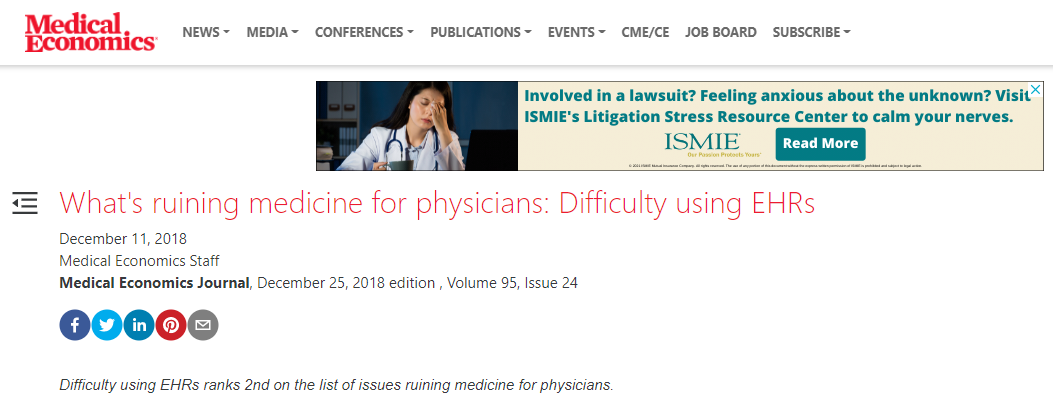
\includegraphics[scale=.3]{graphics/News Clip3.PNG}
\end{center}
\end{frame}

\begin{frame}{This Paper}

Does EHR implementation in hospitals affect labor market decisions of physicians, specifically where, and how much they work?
    
\end{frame}


\section{Contribution}

\begin{frame}{Branches of Literature}
\centering
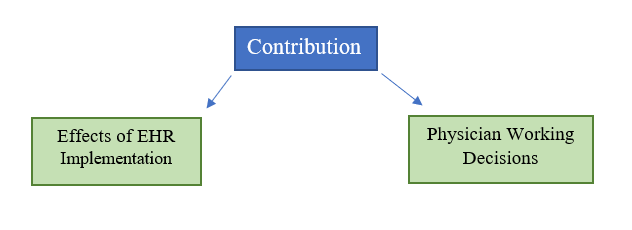
\includegraphics[scale=.45]{graphics/Contribution_litgraphic.PNG}

\end{frame}

\begin{frame}{Physician Labor Literature}
\centering
    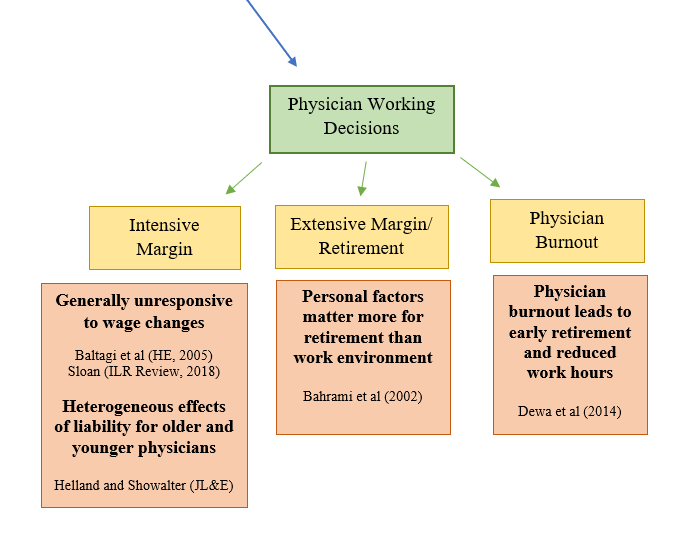
\includegraphics[scale=.45]{graphics/labor_litgraphic.PNG}
\end{frame}

\begin{frame}{EHR Literature}
    \centering
    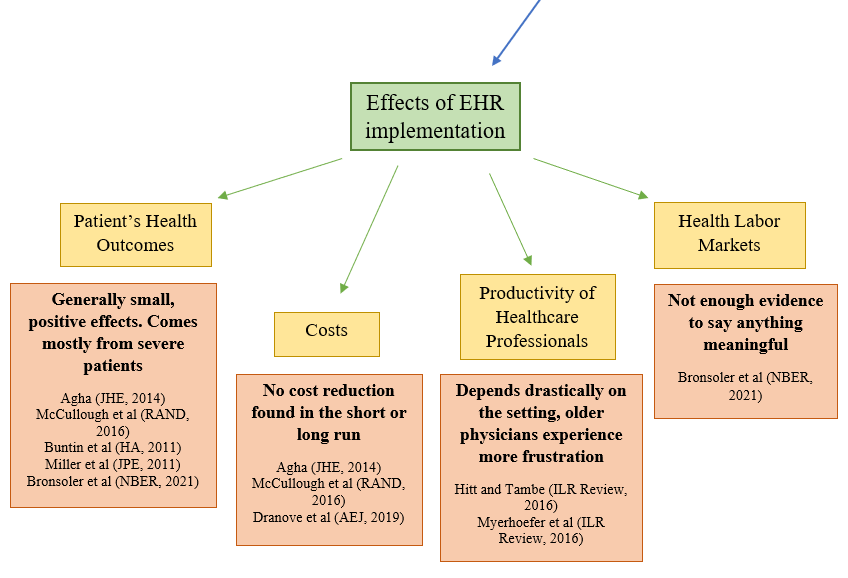
\includegraphics[scale=.45]{graphics/EHR_litgraphic.PNG}
\end{frame}


\section{Model and Data}


\begin{frame}{Physician's Incentives}
\begin{itemize}
    \item Physician decides to work, possibly at a handful of hospitals
    \item Some proportion of these implement a new technology (an EHR)
    \item Two ways to think about the effect:
    \begin{enumerate}
        \item The cost of switching hospitals is higher (attachment to EHR hospital)
        \item The cost of switching hospitals is lower (increased burden at EHR hospital)
    \end{enumerate}
\end{itemize}
\end{frame}


\begin{frame}{Data}
\begin{equation*}
    \textcolor{blue}{p_{iht}}=f(EHR_{ht},EHR_{-h,t},X_i,H_{jt},...)
\end{equation*}

\vspace{3mm}

Measures of physician labor market behavior
\begin{itemize}
    \item Number of shared patients with a hospital: CMS PSPD (2009-2015)
    \item Total services: Medicare Provider Utilization and Payment Data (starts in 2012)
\end{itemize}
\end{frame}

\begin{frame}[noframenumbering]{Data}
\begin{equation*}
    p_{iht}=f(\textcolor{blue}{EHR_{ht},EHR_{-h,t}},X_i,H_{jt},...)
\end{equation*}

\vspace{5mm}

\begin{itemize}
    \item Main variable (binary for whether a hospital uses an EHR) comes from AHA survey
    \item AHA IT Supplement also has information on EHRs that can help with documentation or decision making
    \item Meaningful use data gives information on which hospitals received a subsidy for achieving "meaningful use"
\end{itemize}
\end{frame}

\begin{frame}[noframenumbering]{Data}
\begin{equation*}
    p_{iht}=f(EHR_{ht},EHR_{-h,t},\textcolor{blue}{X_i},H_{jt},...)
\end{equation*}

\vspace{5mm}

Physician level characteristics
\begin{itemize}
    \item Medical school graduation date, gender: Physician Compare
\end{itemize}
\end{frame}

\begin{frame}[noframenumbering]{Data}
\begin{equation*}
    p_{iht}=f(EHR_{ht},EHR_{-h,t},X_i,\textcolor{blue}{H_{jt}},...)
\end{equation*}

\vspace{5mm}

Hospital Level Characteristics
\begin{itemize}
    \item Number of beds: AHA Survey
    \item Number of days out of the year operating: AHA Survey
\end{itemize}
\end{frame}

\begin{frame}{Summary Statistics}
\centering
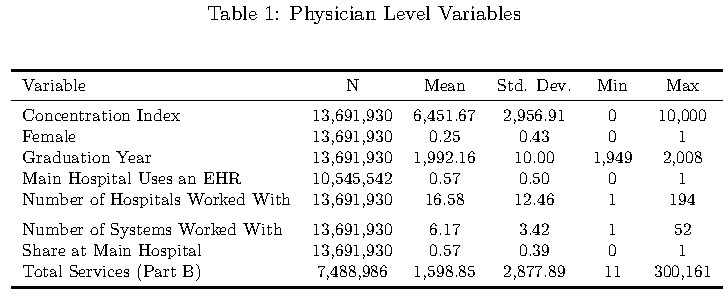
\includegraphics[scale=.45]{Objects/sumstats_physician_table.pdf}\\
\vspace{5mm}
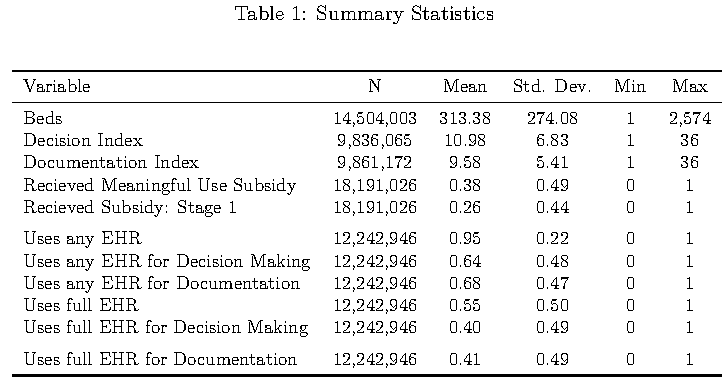
\includegraphics[scale=.45]{Objects/sumstats_pair_table.pdf}\\
\vspace{3mm}
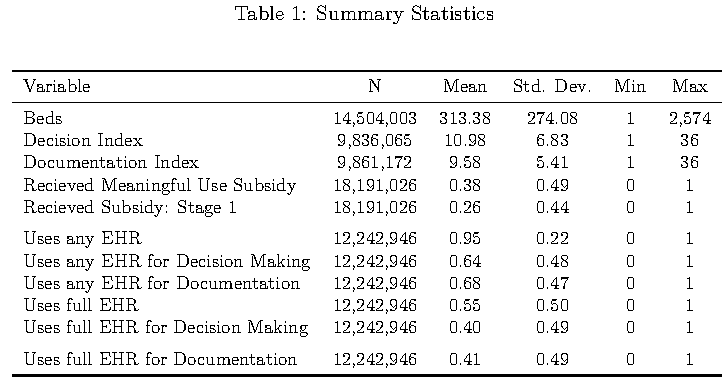
\includegraphics[scale=.45]{Objects/sumstats_hospital_table.pdf}
\end{frame}

\begin{frame}{Variation in EHR Adoption}
\centering
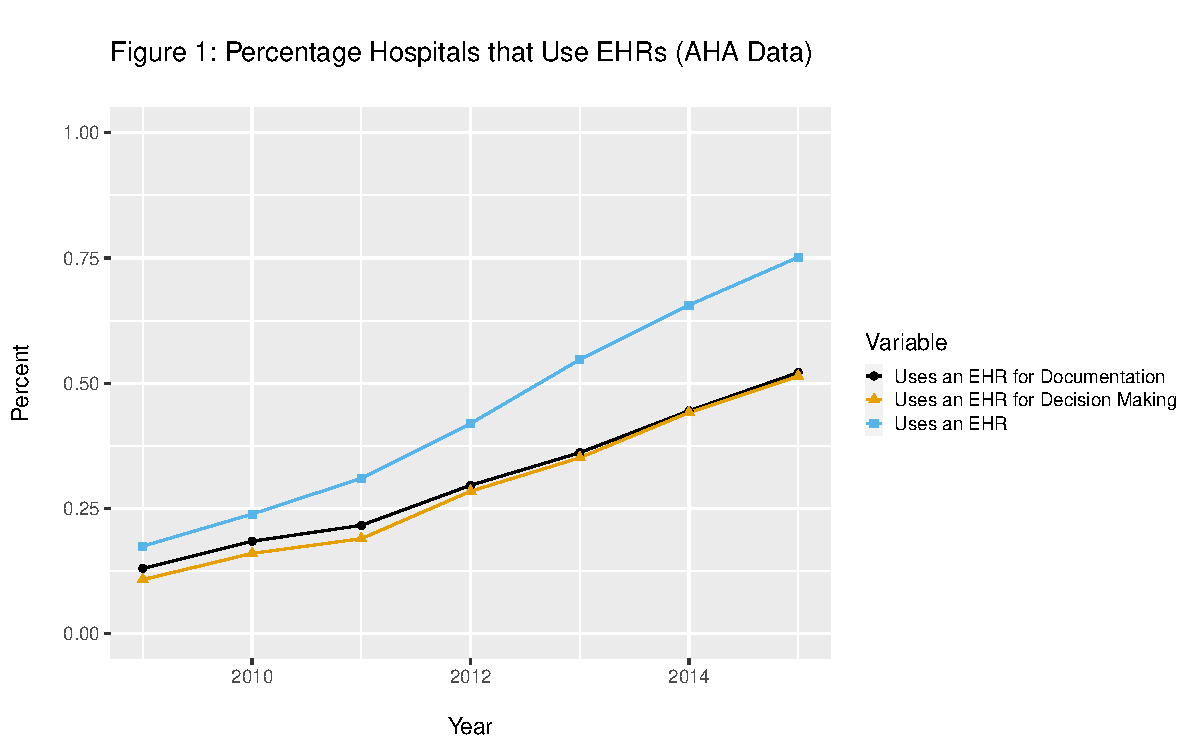
\includegraphics[scale=.55]{Objects/TYP_plot_hospEHR_year.pdf}
\end{frame}





\section{Plans}

\begin{frame}{Original Plan: Difference in Difference}
\begin{itemize}
    \item Treatment: physicians who are exposed to an EHR at one of their hospitals in some year
    \item Control: physicians who are not exposed to a hospital at \textbf{any} hospital in any year
    \begin{itemize}
        \item  Issues with control group because of spillovers
    \end{itemize}
    \item Could still try to attempt this by imposing a control group where the physician has not \textbf{yet} been exposed to an EHR at any hospital
\end{itemize}
\end{frame}

\begin{frame}{Other Ideas}
\begin{itemize}
    \item Aggregate to physician level dataset and do analysis more along the lines of the graph I showed you earlier
    \item Have a continuous measure of EHR use that captures share of exposure to EHRs
\end{itemize}
\end{frame}

\begin{frame}{Miscellaneous Points}
\begin{itemize}
    \item Want to dig deeper into meaningful use measures
    \item Try to get location measurements to think about where physicians are working
    \item Bring in other measures of work from shared patient data
\end{itemize}
    
\end{frame}



\begin{frame}{Variation in Meaningful Use}
    \centering
    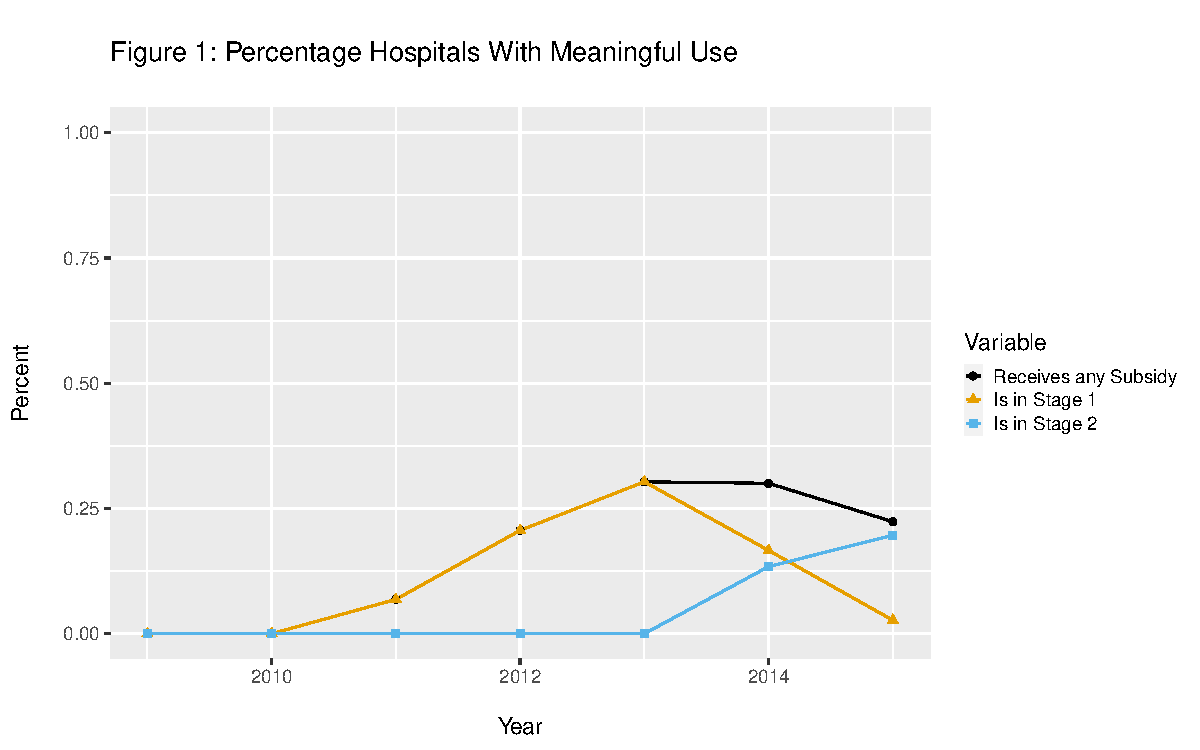
\includegraphics[scale=.5]{Objects/TYP_plot_hospmeanuse_year.pdf}
\end{frame}







\end{document}
